\documentclass[a4paper,10pt]{article}
\usepackage[margin=20mm]{geometry}
\usepackage{fontspec}
% Local editor workaround: fonts are local-only and excluded from distribution.
\IfFileExists{fonts/Arial.ttf}{
\setmainfont[Path=fonts/,BoldFont={Arial Bold.ttf},ItalicFont={Arial Italic.ttf},BoldItalicFont={Arial Bold Italic.ttf}]{Arial.ttf}
}{\setmainfont{Arial}}
\usepackage{amsmath,booktabs,graphicx,array,caption,fancyhdr}
\usepackage[hidelinks]{hyperref}
\captionsetup{font=small,labelfont=bf}
\setlength{\parindent}{0pt}
\setlength{\parskip}{5pt}
\setlength{\tabcolsep}{7pt}
\pagestyle{fancy}\fancyhf{}
\fancyhead[L]{SC4001 Group Project: C analysis}
\fancyhead[R]{11 November 2026}
\fancyfoot[C]{\thepage}
\setlength{\headheight}{14pt}
\begin{document}
{\Large\bfseries Preserving representations under limited-label domain transfer}\par
\textbf{C analysis insert.} These completed experimental sections accompany A/B content. The group must integrate identifiers and its reviewed AI-use declaration into the main report.

\section{Experimental protocol and analysis}
We study whether preserving a pretrained encoder's representations improves sentiment generalization from IMDb movie reviews to Yelp and Amazon reviews. All methods use the same RoBERTa-base revision and a linear classifier on the final-layer CLS representation. The comparison separates freezing (M1), tuning the final two encoder blocks (M2), full fine-tuning (M3), linear probing followed by fine-tuning (M4), low-rank adaptation (M5), feature preservation (M6), and an L2-SP weight-preservation control. M5 trains rank-eight query/value adapters in all 12 layers ($\alpha=16$, no extra adapter dropout) and the classifier: 296,450 trainable parameters. 

Label budgets of 400, 1,600 and 6,400 include both training and validation labels: the corresponding splits contain 320/80, 1,280/320 and 5,120/1,280 examples. Splits are class-balanced, nested within each of five seeds (13, 21, 42, 87, 100), and training and validation remain disjoint across budgets. Source duplicates, conflicting labels and normalized source/test text overlap are removed according to A's fixed preprocessing protocol. Testing uses the unchanged 25,000-example IMDb test set and fixed, deduplicated, balanced 5,000-example target sets for each OOD domain. Target labels define evaluation samples only; they do not select hyperparameters.

Every candidate trains for ten epochs in FP32, with maximum length 512, batch size eight, four-step gradient accumulation, AdamW weight decay 0.01 and warmup ratio 0.1. Epoch and candidate selection use IMDb validation accuracy, with fixed tie rules. M6 and L2-SP inherit the selected M3 learning rate and search three penalty coefficients. M4 additionally trains a first-stage linear probe using A's selected M1 learning rate. Equal numbers of second-stage candidates therefore do not imply equal total search cost. M5 searches learning rates $10^{-4}$, $3\times10^{-4}$ and $10^{-3}$; complete grids and pilot history remain in the frozen protocols.

The primary outcome is the equal mean of Yelp and Amazon accuracy, computed within each seed before aggregation. Paired differences use the same budget and seed. We report sample standard deviations and approximate, unadjusted 95\% paired-$t$ intervals; five seeds are insufficient to verify their distributional assumptions. Exact two-sided sign-flip tests enumerate all $2^5$ assignments, with minimum attainable $p=0.0625$. Holm adjustment is applied separately to the three focal M6--M3 OOD comparisons, 69 original secondary contrasts and 18 later M5 contrasts. These analyses were designed after the A/B results were available and are exploratory, not retrospectively preregistered confirmation. Test examples, domains and layers are not additional training replicates.

\section{Accuracy and uncertainty}
\begin{center}
\begin{tabular}{lrrr}\toprule
Method & Budget 400 & Budget 1,600 & Budget 6,400\\\midrule
M1 & 82.74 $\pm$ 3.48 & 87.47 $\pm$ 0.85 & 89.91 $\pm$ 1.02 \\
M2 & 91.53 $\pm$ 0.87 & 92.45 $\pm$ 1.07 & 93.88 $\pm$ 0.49 \\
M3 & 92.73 $\pm$ 0.75 & 92.21 $\pm$ 1.28 & 93.89 $\pm$ 0.54 \\
M4 & 91.78 $\pm$ 2.48 & 93.14 $\pm$ 1.30 & 94.36 $\pm$ 0.87 \\
M6 & 92.03 $\pm$ 0.68 & 92.90 $\pm$ 0.77 & 93.92 $\pm$ 0.61 \\
L2-SP & 92.38 $\pm$ 1.05 & 92.71 $\pm$ 2.12 & 94.23 $\pm$ 0.64 \\
\bottomrule\end{tabular}

\captionof{table}{OOD accuracy (\%), mean $\pm$ sample SD over five paired seeds. OOD is the equal mean of the two fixed target domains. All candidates and checkpoints are selected using IMDb validation accuracy only.}
\end{center}
M1 remains below encoder-adaptation methods. At budget 6,400, M2 and M3 reach 93.880\% and 93.886\% OOD accuracy, although M2 trains 14.18 million rather than 124.06 million parameters. M3 and M4 have the highest observed means at budgets 400 and 6,400; M5 leads M4 by only 0.012 points at 1,600. These rankings do not establish population-wide superiority.

\clearpage
\section{Representation preservation and generalization}
M6--M3 mean OOD differences are $-0.702$, $+0.694$ and $+0.038$ percentage points at the three increasing budgets. Their paired-$t$ intervals are $[-1.643,0.239]$, $[-1.520,2.908]$ and $[-0.399,0.475]$, respectively. M6 wins in only one, two and three of the five paired seeds. The positive mean at budget 1,600 is therefore not a majority-seed improvement. Exact Holm-adjusted $p$ values are 0.375, 1.000 and 1.000. These results provide no stable evidence that M6 improves OOD accuracy over full tuning; they do not establish equivalence.

For sensitivity, 10,000 bootstrap replicates preserve example pairing across methods and seeds. Conditional fixed-model intervals omit variation from retraining and are therefore narrower. At budget 400, a crossed seed/example percentile interval is $[-1.332,-0.086]$ percentage points, whereas the paired-$t$ interval crosses zero. We disclose this small-sample method sensitivity rather than select the interval giving the strongest conclusion. At budgets 1,600 and 6,400, crossed intervals also span zero.

Representation diagnostics use 256 deterministically selected, class-balanced examples per domain, identical across checkpoints. We compute linear centered kernel alignment (CKA), a debiased sensitivity estimate, a fixed input-permutation control and cosine distance. Both CLS states and non-padding-token means are evaluated at the embedding output and all 12 encoder layers. Mean pooling includes special tokens. Each trained representation is compared with the original pretrained encoder; M4, M6 and L2-SP are additionally compared with paired M3 checkpoints. CKA measures geometry, not semantic correctness or a causal mechanism \cite{cka}.

\begin{center}
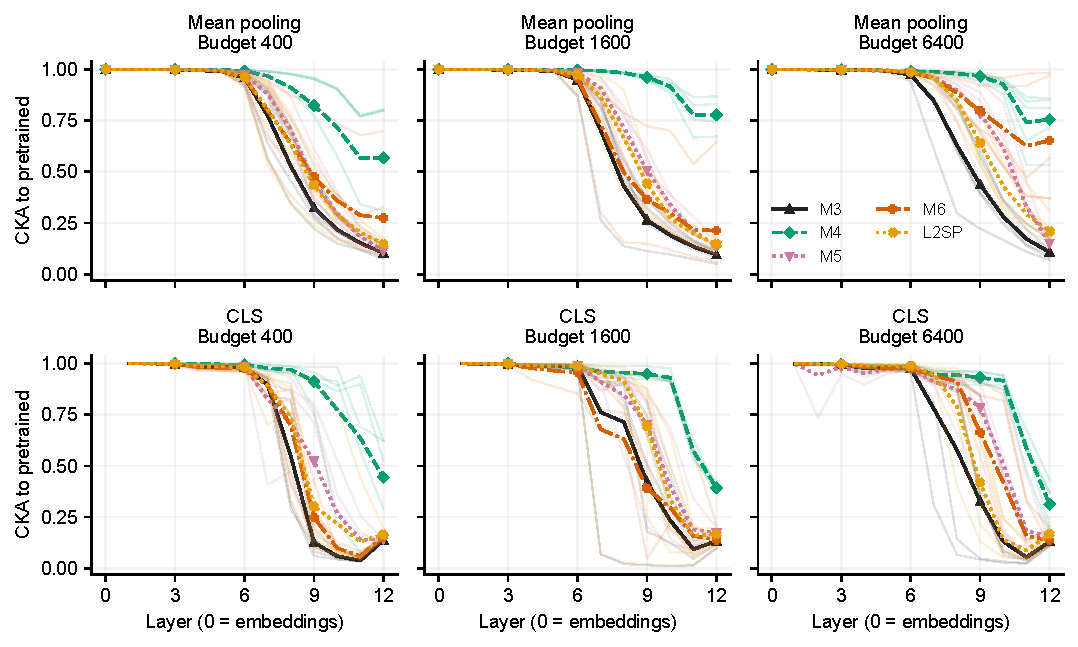
\includegraphics[width=\linewidth]{images/02_cka_layers.pdf}
\captionof{figure}{OOD CKA to the pretrained encoder, averaging Yelp and Amazon within each seed. Thin lines retain individual-seed variation; thick lines show means. Rows distinguish mean pooling and CLS. Constant layer-0 CLS representations have undefined CKA and are omitted, not treated as perfect agreement.}
\end{center}
M6 raises mean-pooled last-layer OOD CKA from M3's 0.104, 0.095 and 0.108 to 0.274, 0.213 and 0.652. The corresponding debiased values retain this pattern (M3: 0.088, 0.080, 0.093; M6: 0.259, 0.199, 0.643), and exceed the shuffled-control means (M6: 0.018, 0.015, 0.025). This supports measurable representation preservation. It does not imply improved classification: accuracy differences remain mixed across budgets and seeds.

The effect is pooling-dependent. M6's final CLS CKA remains close to M3's, whereas its penalty directly anchors the token mean. A plausible explanation is that preserving pooled sentence geometry does not sufficiently constrain the CLS feature used by the classifier. This is an interpretation of the observed mismatch, not a tested causal account. M5 mean-pooled last-layer OOD CKA is only 0.116, 0.137 and 0.150 (debiased: 0.099, 0.118 and 0.132). Training few parameters therefore does not guarantee preservation of this representation geometry.

\clearpage
\section{Ablation and error analysis}
M4 also preserves mean-pooled geometry (last-layer OOD CKA 0.569, 0.778 and 0.755), without explicitly imposing M6's penalty. L2-SP produces smaller changes in this metric (0.147, 0.145 and 0.209). Preservation is therefore not unique to M6, and its extent alone does not order OOD performance. Within-method, within-budget rank correlations use only five seeds and are descriptive; pooling methods or budgets would confound adaptation strategy, data availability and penalty selection.

\begin{center}
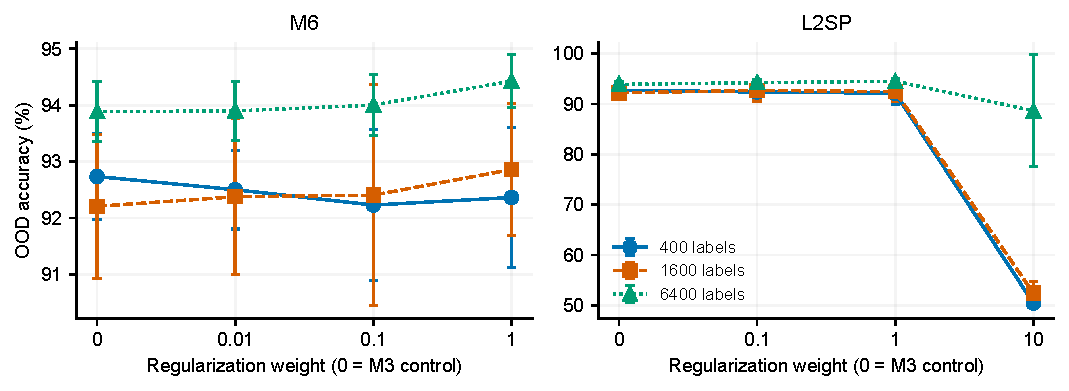
\includegraphics[width=\linewidth]{images/04_lambda_ablation.pdf}
\captionof{figure}{Predefined penalty sweeps. Points and bars show mean OOD accuracy and sample SD across five seeds. Target evaluations describe all predefined penalty candidates; they never replace the source-validation selection rule. Coefficient scales differ between the cosine and summed squared-weight penalties and are not numerically comparable.}
\end{center}
M6 selects $\lambda=0.01/0.1/1$ in 1/3/1, 4/0/1 and 1/2/2 seeds at budgets 400, 1,600 and 6,400. L2-SP selects its smallest coefficient, 0.1, in 14 of 15 cells. Selected-model averages thus mix different regularization strengths. In M6's budget-6,400 runs, three-domain last-layer mean CKA ranges from about 0.35 to 0.99; the two seeds choosing $\lambda=1$ are near 0.98--0.99. Reporting only the mean would conceal this heterogeneity. The absence of $\lambda=0$ from the penalty grids also matters: M3 is a separate control, not an available fallback during M6/L2-SP selection.

Error analysis compares M6 and M3 on identical examples, separating shared successes, shared errors, fixes and regressions. At budget 400, M6's Amazon accuracy change is $-2.008$ percentage points for negative examples and $+0.072$ for positive examples. At budget 1,600, negative-class changes are positive on both targets (+1.424 points on Yelp, +1.104 on Amazon), while positive-class changes are smaller. Aggregate gains or losses can mask class-specific shifts; these observations do not establish why the shifts occur.

Long inputs remain a limitation of the 512-token protocol. On IMDb at budget 6,400, M3 averages 92.28\% on inputs longer than 512 tokens versus 94.79\% on inputs of 129--512 tokens. These groups differ in content and difficulty, so the gap is not a causal estimate of truncation damage. Sparse strata require further restraint: the Amazon greater-than-512 group contains only one example and is not a reliable subgroup benchmark. Negation-marker groups are simple lexical heuristics, not expert linguistic annotations.

Error transitions are also seed-dependent. At budget 1,600, 118 Yelp examples and 141 Amazon examples are fixed in at least one seed but broken in another. Only four Yelp examples and three Amazon examples are fixed in at least three seeds. A favorable anecdote is therefore weak evidence for a robust mechanism. The case file selects one example per correctness-transition category using a fixed hash rule, across all budgets and domains at seed 13. It retains IDs, text hashes and short excerpts. AI-assisted interpretations remain pending team review and are not presented as human-coded evidence.

\clearpage
\section{Computational cost and practical trade-offs}
We distinguish complete training records, hyperparameter search, short computational probes and inference. Source records retain selected-run and incremental-search time. Standalone reproduction additionally includes inherited M3 search for M6/L2-SP and M1 search for M4. Shared searches must not be counted repeatedly in the actual project's total. One nonselected M6 candidate (budget 6,400, seed 21, $\lambda=1$) resumed after timeout; its stored training time covers only the final invocation. Search-time totals for that cell are lower bounds. The selected $\lambda=0.01$ model was not resumed.

The original B implementation kept a diagnostic pretrained teacher on the GPU for M3, M4 and L2-SP, although their losses do not require it. We retain the clean Tesla V100-PCIE-32GB probes and add matched RTX 6000 Ada probes covering all seven methods. Each uses the same 32 source-training examples already tokenized and resident on the GPU, length 512, batch eight, accumulation four and FP32 with TF32 disabled. Two optimizer steps warm up the process and five steps are timed; three independent processes estimate measurement variability. These process repeats are not additional model seeds.

\begin{center}
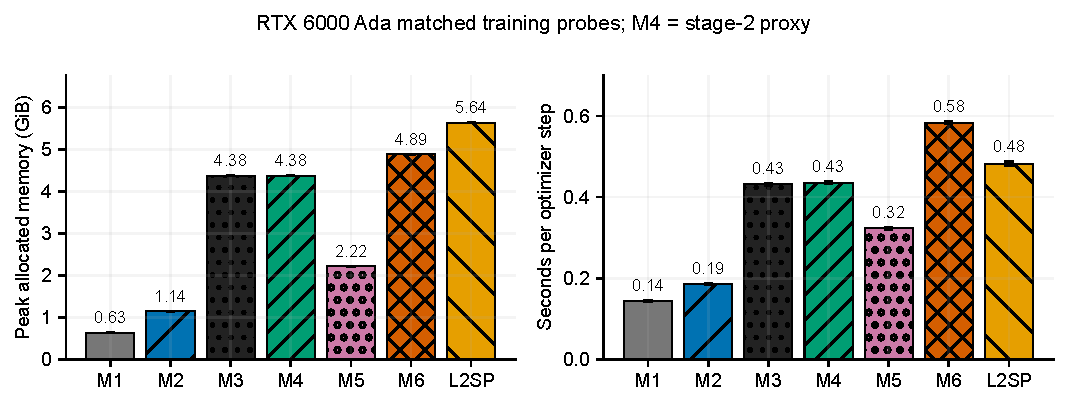
\includegraphics[width=\linewidth]{images/06_ada_cost.pdf}
\captionof{figure}{Matched fixed-shape RTX 6000 Ada training probes, three fresh processes per method. M6 retains the teacher required by its objective; L2-SP retains its reference-weight snapshot. M4 is a second-stage compute proxy, not the cost of its complete two-stage procedure. Peaks are allocated GPU tensor memory, not total device occupancy or a guaranteed provisioning limit.}
\end{center}
On Ada, M3 uses 4.376 GiB peak allocated memory and 0.432 seconds per optimizer step. M5 uses 2.220 GiB and 0.323 seconds: about 49.3\% less memory and 25.3\% less step time. Its 0.24\% trainable-parameter fraction does not imply a proportional computational reduction. M6 uses 4.892 GiB and 0.584 seconds; L2-SP uses 5.642 GiB and 0.483 seconds. These are implementation-specific, short training probes.

M1 and M2 remain cheaper on Ada (0.628 and 1.142 GiB; 0.143 and 0.185 seconds per step). M2 closely matches M3 at the largest budget. M5 uses about 94.5\% more memory and 74.2\% more step time than M2, while its budget-6,400 OOD advantage is only 0.176 points (paired interval $[-0.394,0.746]$). LoRA reduces optimizer state, but adapters throughout the encoder still require backward computation; parameter count alone does not rank actual cost. M6's additional cost likewise lacks a consistent accuracy advantage.

The archived inference probe uses a fresh pretrained encoder and seeded classifier rather than trained winners. Its common throughput of about 112 examples/second characterizes the shared architecture at a fixed input shape; it is not a deployment comparison. M5's 45 candidate-training invocations total 3.492 hours on Ada, including in-training validation and saving; no candidate resumed. This excludes testing, diagnostic jobs and outer-process overhead. Full-training times remain separate from V100 timings. The adapter inference probe is unmerged, so it is not a measurement of trained, merged-model deployment. No cross-hardware speedup is claimed.

\clearpage
\section{Discussion and limitations}
The evidence distinguishes two propositions. First, feature preservation changes measured geometry: M6 increases mean-pooled CKA relative to full fine-tuning. Second, preserved geometry need not improve target classification: M6's paired OOD effects vary in sign and seed stability, and it incurs additional training cost. This study supports a conditional, measurement-specific account of preservation, rather than a general claim that closer pretrained representations necessarily transfer better.

The design draws on source-only model selection and regularization from the course, and on prior transfer-learning work. LP-FT motivates staged adaptation \cite{lpft}; L2-SP anchors parameters to the pretrained solution \cite{l2sp}; DELTA motivates feature-space preservation in a different architecture with a different attention mechanism \cite{delta}. Our pooled cosine penalty is not an implementation of DELTA, and the vision results in those papers do not themselves validate a claim about review sentiment transfer.

Several limitations restrict interpretation. Five paired seeds provide low inferential resolution and share a common source pool and fixed test sets; they do not sample the universe of possible domains. Only one encoder family and two target review domains are studied. Target sets are balanced by design, so results need not transfer to naturally imbalanced deployment traffic. The length cap can remove relevant content. CKA depends on inputs, pooling and layer, and a fixed 256-example subset cannot capture all behavior. Source-validation accuracy may favor a different penalty from target accuracy; target-guided reselection would invalidate the protocol. Candidate searches are bounded rather than exhaustive, and inherited searches make their costs unequal. The analyses are exploratory and informed by existing A/B outcomes.

\textbf{Parameter-efficient adaptation.} LoRA is an established comparator \cite{lora}. M5--M3 OOD differences are $-1.670$, $+0.946$ and $+0.170$ points; paired intervals are $[-5.060,1.720]$, $[-1.595,3.487]$ and $[-0.626,0.966]$. M5 wins in three, two and three seeds, respectively; all three exact Holm-adjusted $p$ values are 1.000. At budget 400, its OOD SD is 2.669 points and seed 42 reaches only 87.34\% OOD accuracy. This failure is retained. Four of five low-budget selections use the highest prespecified learning rate, so the bounded search is a limitation, not justification for target-guided expansion. At 1,600, M5's 0.012-point mean lead over M4 is negligible relative to seed variation. LoRA provides a measured resource trade-off against full tuning, not a universal accuracy or efficiency advantage.

\textbf{Evidence and reproducibility.} The A/B audit covers 285 candidate-training records and 450 prediction files, including predefined penalty ablations. The GPU supplement covers 60 selected B checkpoints, 8,190 CKA rows and 27 cost probes. Its 180 checkpoint-probability replay checks pass a $10^{-4}$ tolerance; the largest discrepancy is $8.03\times10^{-5}$. All 244 return-manifest file hashes match. Constant layer-0 CLS states account for 315 expected undefined CKA entries. The return records checkpoint weight hashes, but local review did not download and independently hash B's complete weight archive. The independent M5 return audit checks all 809 manifested files, 45 prediction files (525,000 rows), 15 source choices and 18 paired contrasts; the statistical tables reproduce exactly. M5 adds 1,170 CKA rows, 45 probability replays and 21 matched Ada probes. Its 45 undefined layer-0 CLS entries are expected. Code, manifests, per-seed tables and commands are retained separately from large weights and caches.

\textbf{AI use statement for team review.} Codex assisted with audit and analysis code, LoRA implementation, experiment orchestration, statistical interpretation, figures and drafting these C sections. Earlier planning also involved Claude, as reported in the project conversation; the team should confirm its exact scope in the consolidated declaration. Numerical claims here are linked to actual A/B records and completed M5 GPU experiments. Synthetic local tests are labeled as such. The team remains responsible for reviewing explanations, references and case interpretations, understanding the code and ensuring the submission follows course rules. No unrecorded human review is claimed.

\textbf{Integration note.} These sections reserve five main-text pages for C. Consolidate it with A/B's introduction, related work, model definitions and data description so the entire report remains within ten main-content pages. The group must supply identifiers, review these sections and integrate A/B content. External coursework comparison and final package checks are documented separately from the scientific results. No grade or full-mark outcome is asserted.

\clearpage
\begin{thebibliography}{9}
\bibitem{cka} S. Kornblith, M. Norouzi, H. Lee and G. Hinton. Similarity of Neural Network Representations Revisited. ICML, PMLR 97:3519--3529, 2019. \url{https://proceedings.mlr.press/v97/kornblith19a.html}.
\bibitem{lpft} A. Kumar, A. Raghunathan, R. Jones, T. Ma and P. Liang. Fine-Tuning can Distort Pretrained Features and Underperform Out-of-Distribution. ICLR, 2022. \url{https://arxiv.org/abs/2202.10054}.
\bibitem{l2sp} X. Li, Y. Grandvalet and F. Davoine. Explicit Inductive Bias for Transfer Learning with Convolutional Networks. ICML, 2018. \url{https://arxiv.org/abs/1802.01483}.
\bibitem{delta} X. Li, H. Xiong, H. Wang, Y. Rao, L. Liu, Z. Chen and J. Huan. DELTA: DEep Learning Transfer using Feature Map with Attention for Convolutional Networks. ICLR, 2019. \url{https://arxiv.org/abs/1901.09229}.
\bibitem{lora} E. J. Hu, Y. Shen, P. Wallis, Z. Allen-Zhu, Y. Li, S. Wang, L. Wang and W. Chen. LoRA: Low-Rank Adaptation of Large Language Models. 2021. \url{https://arxiv.org/abs/2106.09685}.
\end{thebibliography}
\clearpage
\appendix
\section{Domain-specific diagnostics}
\begin{center}
{\fontsize{8.5}{10}\selectfont\setlength{\tabcolsep}{3.5pt}\begin{tabular}{rlrrrrr}\toprule
Budget & Domain & M3 mean CKA & M6 mean CKA & $\Delta$ CLS CKA & $\Delta$ cosine & $\Delta$ acc. (pp)\\\midrule
400 & IMDb & 0.046 & 0.220 & +0.007 & -0.252 & -0.059 \\
400 & Yelp & 0.096 & 0.311 & +0.015 & -0.205 & -0.436 \\
400 & Amazon & 0.112 & 0.237 & +0.015 & -0.219 & -0.968 \\
1600 & IMDb & 0.039 & 0.175 & +0.000 & -0.364 & +0.273 \\
1600 & Yelp & 0.087 & 0.243 & +0.007 & -0.303 & +0.692 \\
1600 & Amazon & 0.103 & 0.183 & +0.005 & -0.310 & +0.696 \\
6400 & IMDb & 0.049 & 0.638 & +0.003 & -0.428 & +0.081 \\
6400 & Yelp & 0.105 & 0.724 & +0.003 & -0.348 & -0.052 \\
6400 & Amazon & 0.110 & 0.581 & +0.007 & -0.362 & +0.128 \\
\bottomrule\end{tabular}
}
\captionof{table}{Last-layer diagnostics and full-test accuracy, averaged across five paired seeds. All differences are M6 minus M3. Cosine distance uses non-padding mean representations; lower distance indicates closer pointwise alignment to the pretrained reference. CKA and accuracy have different scales.}
\end{center}
The pooled-geometry effect is visible separately in source and target domains, rather than arising only from averaging Yelp and Amazon. At budget 6,400, mean-pooled cosine distance falls from 0.385 to 0.023 on Amazon and from 0.370 to 0.022 on Yelp. Yet their accuracy changes are only +0.128 and -0.052 percentage points. CLS CKA changes remain small. The CLS cosine distance nevertheless decreases (Amazon: 0.540 to 0.296; Yelp: 0.532 to 0.281), illustrating that the conclusion depends on which aspect of representation similarity is measured. We do not interpret any of these quantities as a semantic fidelity score.

\begin{center}
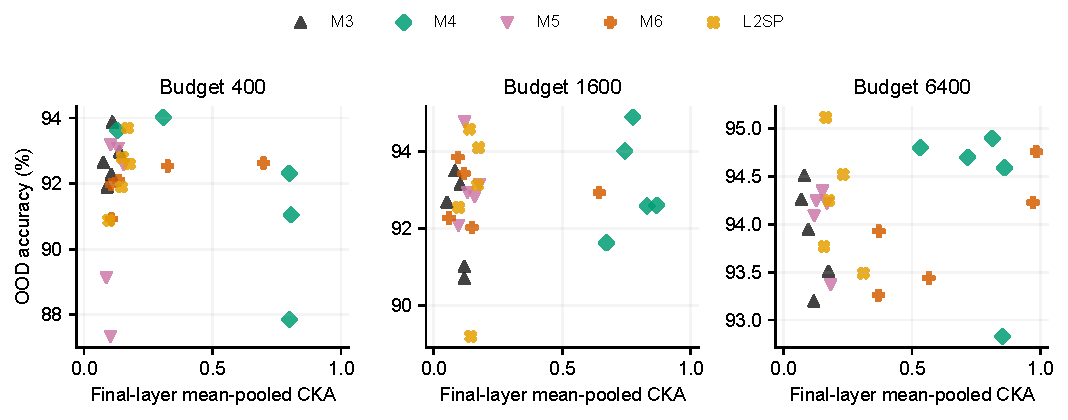
\includegraphics[width=.94\linewidth]{images/03_cka_accuracy.pdf}
\captionof{figure}{Each point is one selected model seed; OOD domains are averaged within that seed. Keeping budgets separate avoids conflating additional labels with representation preservation. No pooled regression or causal trend is asserted.}
\end{center}

\begin{center}
\begin{tabular}{rlrrr}\toprule
Budget & Domain & $\Delta$ Brier & $\Delta$ NLL & $\Delta$ ECE\\\midrule
400 & IMDb & -0.0033 & -0.0644 & -0.0125 \\
400 & Yelp & +0.0004 & -0.0250 & -0.0130 \\
400 & Amazon & +0.0049 & -0.0177 & -0.0091 \\
1600 & IMDb & -0.0010 & +0.0120 & +0.0035 \\
1600 & Yelp & -0.0037 & -0.0068 & +0.0059 \\
1600 & Amazon & -0.0039 & -0.0024 & +0.0021 \\
6400 & IMDb & -0.0015 & -0.0154 & -0.0022 \\
6400 & Yelp & -0.0012 & -0.0301 & -0.0065 \\
6400 & Amazon & -0.0028 & -0.0415 & -0.0066 \\
\bottomrule\end{tabular}

\captionof{table}{Probability-quality differences, M6 minus M3; negative values indicate smaller loss or calibration error. Brier and binary NLL are computed from the archived probabilities; NLL clips probabilities to $[10^{-12},1-10^{-12}]$. ECE uses 15 equal-width top-label confidence bins and is descriptive. No calibration model is fitted.}
\end{center}
Probability quality can diverge from accuracy: at budget 400, Amazon Brier worsens while NLL and ECE improve; at budget 1,600, ECE worsens in all domains despite positive mean accuracy changes. These descriptive diagnostics do not justify target-based recalibration or model selection.

\clearpage
\section{Hardware and diagnostic scope}
\begin{center}
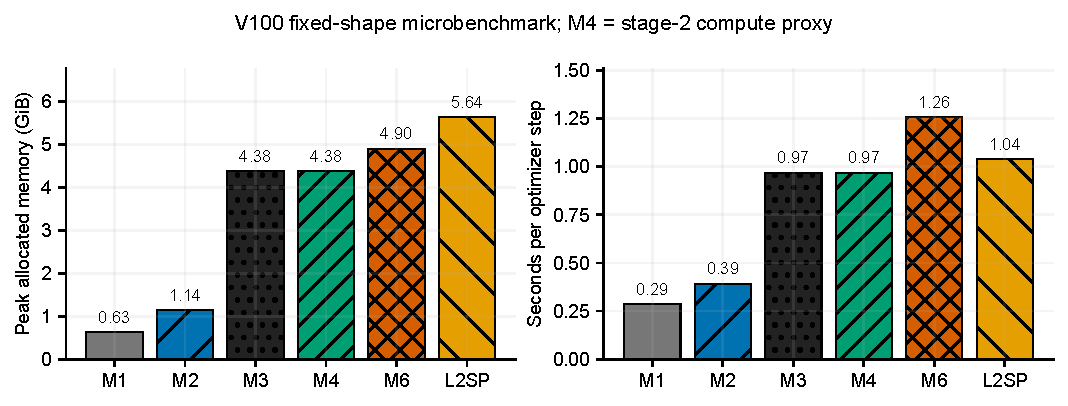
\includegraphics[width=\linewidth]{images/05_v100_cost.pdf}
\captionof{figure}{Archived clean V100 probes, retained as a separate hardware stratum. These results must not be divided into the Ada timings to infer an adaptation-method speedup.}
\end{center}
Representation diagnostics cover M3, M4, M5, M6 and L2-SP; M1/M2 comparisons use accuracy and cost. M5 CKA uses Ada and a pretrained reference only, whereas B diagnostics on V100 also include direct paired-M3 references. Inputs, FP32 precision and estimators are matched, but small hardware-dependent numerical differences remain possible.

On V100, M3 uses 4.377 GiB and 0.969 seconds per step; M6 uses 4.899 GiB and 1.257 seconds (11.9\% more memory and 29.7\% more time). The unnecessary diagnostic teacher raises M3/M4 peak allocation by about 0.472 GiB. The fresh-pretrained inference probe characterizes a shared architecture, not trained model deployment. M4 probes only its second stage; its first-stage training and inherited M1 search remain part of full accounting.
\end{document}
